\chapter{Estado del arte}
\label{cap:capitulo2}
En este capítulo se expone el estado del arte de los robots industriales en educación. Esta fase fundamental de la 
investigación se ha completado gracias a la búsqueda en diversas fuentes de renombre, con el fin de 
recopilar información que pueda ser de utilidad para desarrollar el presente proyecto de fin de grado. Como resultado, se 
han seleccionado una serie de trabajos relevantes y significativos en la materia, que se procederán a analizar a continuación.
\begin{itemize}
    \item En \cite{KRIMPENIS2020103} se presenta una solución industrial barata para crear un robot capaz de hacer operaciones de mecanizado (fabricación 
    de piezas mediante operaciones de corte). Es llamado Hydra y esta dotado de 6 \ac{DOF}. Tiene un alcance máximo de casi un metro y un 
    peso que ronda los 13 Kg. Pese a todas estas funciones, está fabricado mediante impresión 3D. 
    Además, tiempo después, se publicó la segunda parte de este artículo: \cite{PAPAPASCHOS2020109}. En el cual se aborda el diseño software y de control 
    que se ha desarrollado para controlar dicho brazo. \\
    \begin{figure} [h!]
        \begin{center}
          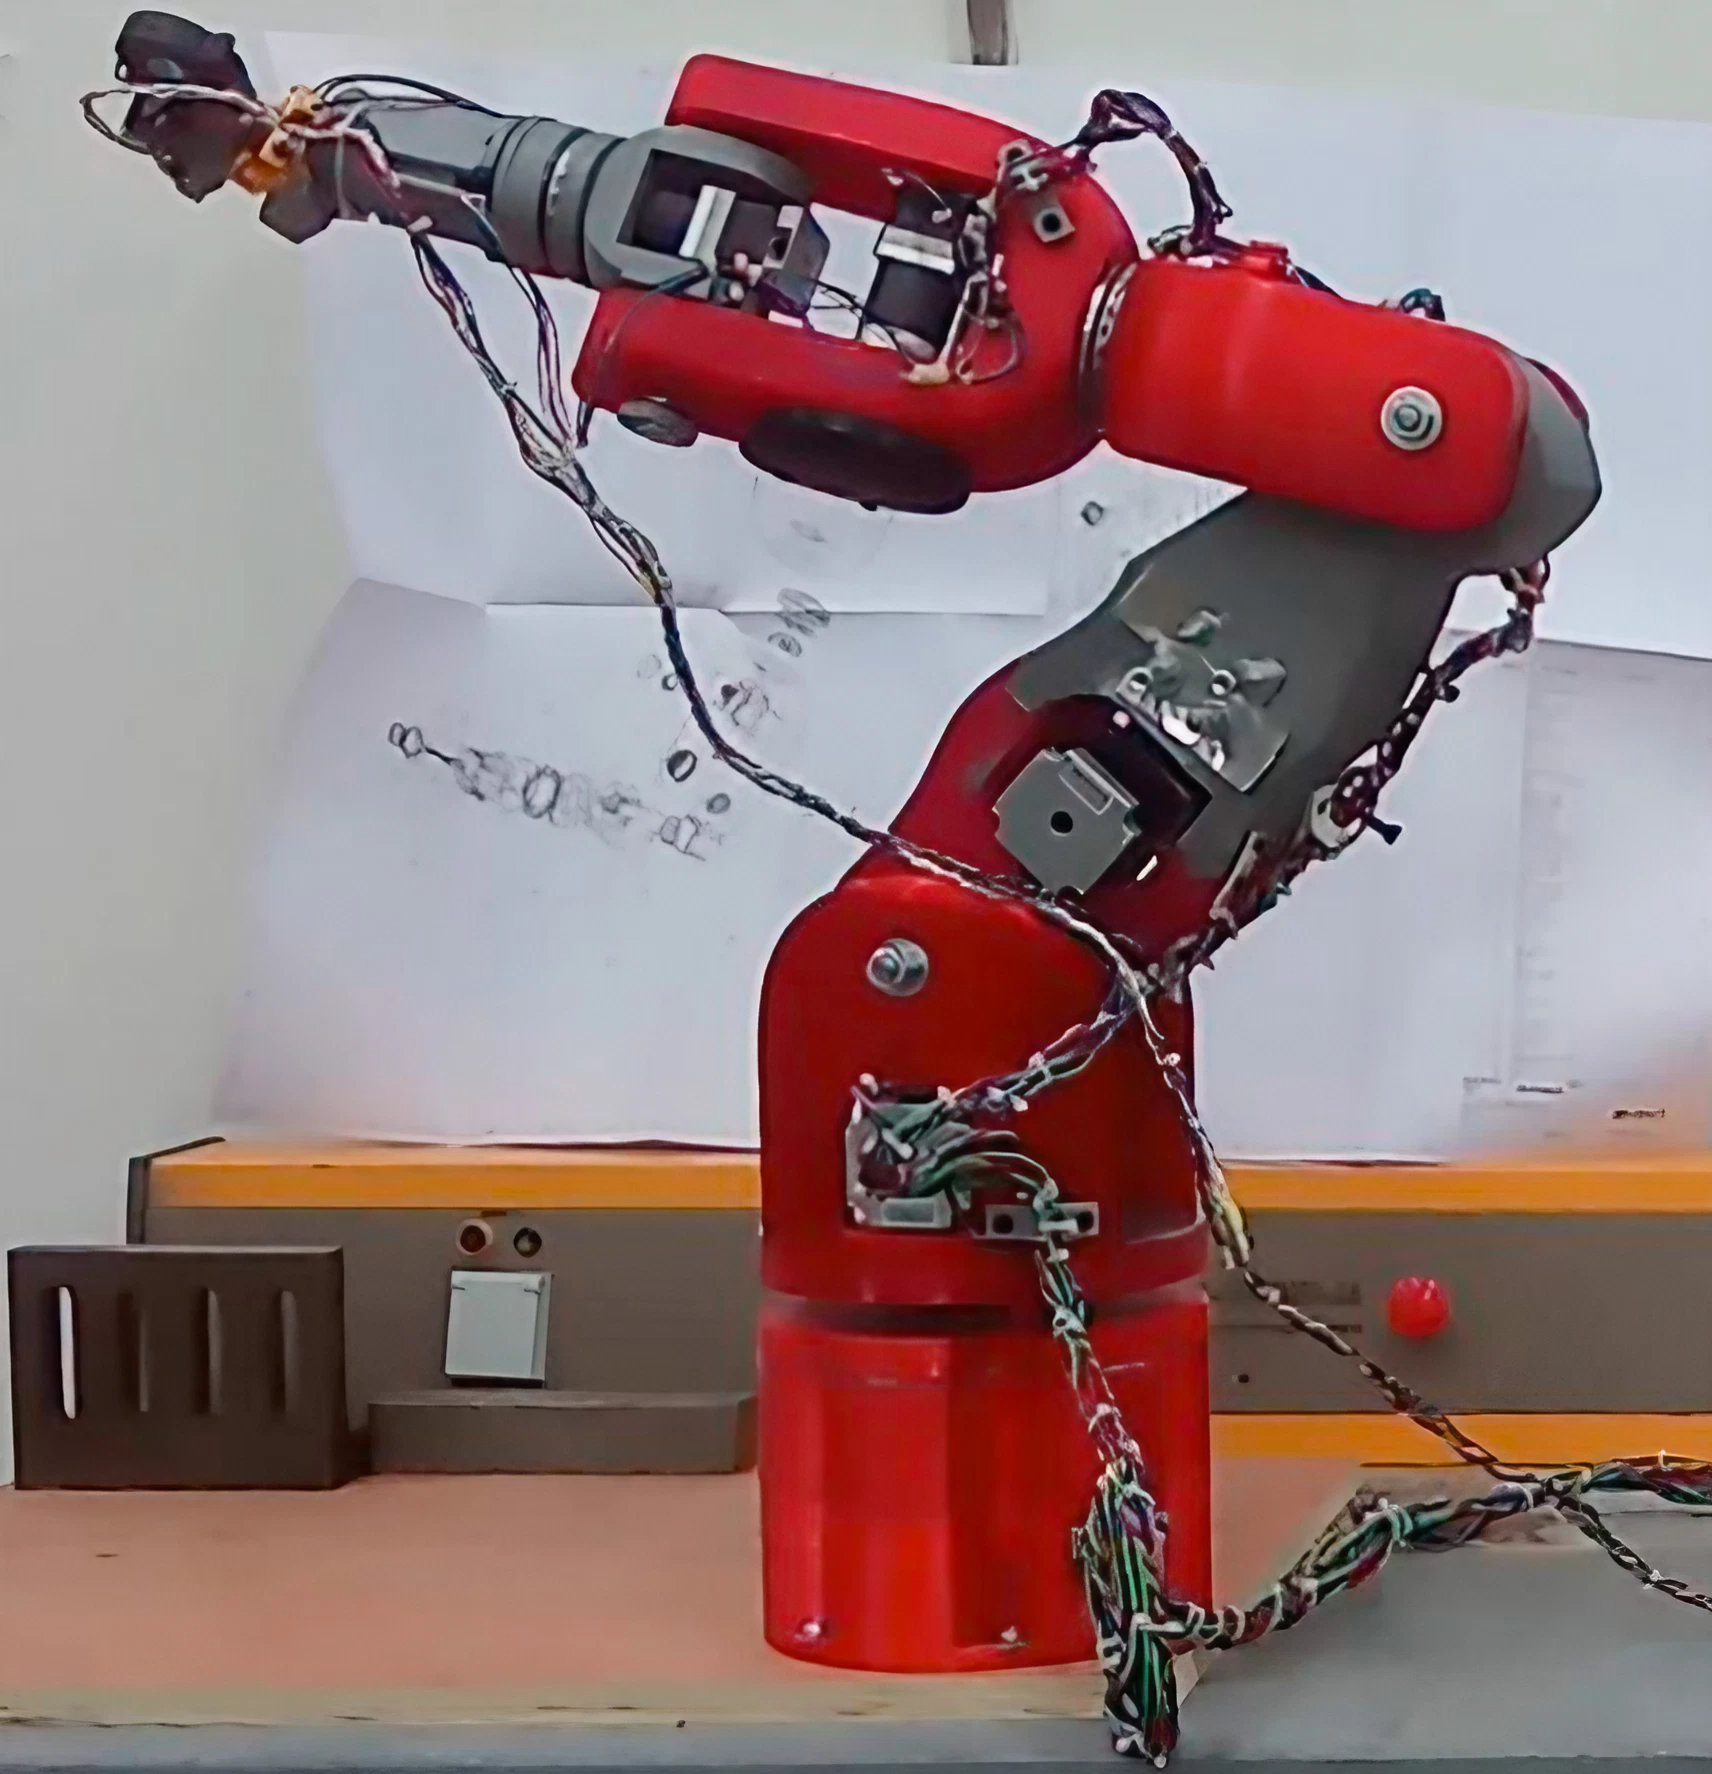
\includegraphics[width=6cm]{figs/Hydra.png}
        \end{center}
        \caption{Robot HydraX}
        \label{fig:hydra}
    \end{figure}\ 
    \newpage
    En base a lo descrito en estos artículos se han extraído los siguientes puntos fuertes del proyecto:
    \begin{itemize}
        \item Tiene una repetitividad de ±0.04 mm.
        \item Tiene un espacio de trabajo muy amplio.
        \item Tener más de 3 grados de libertad le permiten alcanzar gran cantidad de puntos con distintas orientaciones.
        \item Según el artículo, tiene una capacidad de carga máxima de 12 kilogramos. A pesar de esto, se comenta que en la práctica el peso en el 
        extremo del robot debe ser menor a 5 Kg, por lo que su carga útil rondará los 3 Kg para un funcionamiento aceptable. Esto lo sitúa a la par 
        del robot comercial ABB IRB 120\footnote{\url{https://new.abb.com/products/es/3HAC031431-001/irb-120}}  
    \end{itemize}\
    
    En cambio, también se deben mencionar los siguientes puntos débiles:
    \begin{itemize}
        \item Carece de integración en \ac{ROS}, plataforma de desarrollo de la que se habla en \ref{subsec:ros2}
        \item Su coste en materiales supera los 1000 \euro \xspace por lo que no es lo suficientemente asequible para su uso académico.
        \item Según este artículo, se necesitan 200 horas para poder imprimir y montar el brazo, lo que implica que es costoso en tiempo 
        crear varias unidades y requiere de cierta habilidad para construirlo correctamente.
        \item En este artículo no se proporcionan los ficheros necesarios para poder replicarlo. Además, se menciona que las piezas han sido 
        diseñadas mediante el software privativo SolidWorks\textsuperscript{\tiny\textregistered} por lo que lo hace más difícil y costoso de editar.
    \end{itemize}\
    \newpage
    \item Existen soluciones más sencillas y reproducibles, como por ejemplo, la presentada en \cite{adediran2023uiarm}. Se trata de un brazo robótico 
    cuyo propósito es separar botellas de plástico en un proceso de reciclaje. Más allá de la aplicación que se le pretende dar, se hace uso de  
    un manipulador de tamaño reducido, impreso en 3D y con 4 \ac{DOF}.
    \begin{figure} [ht!]
        \begin{center}
          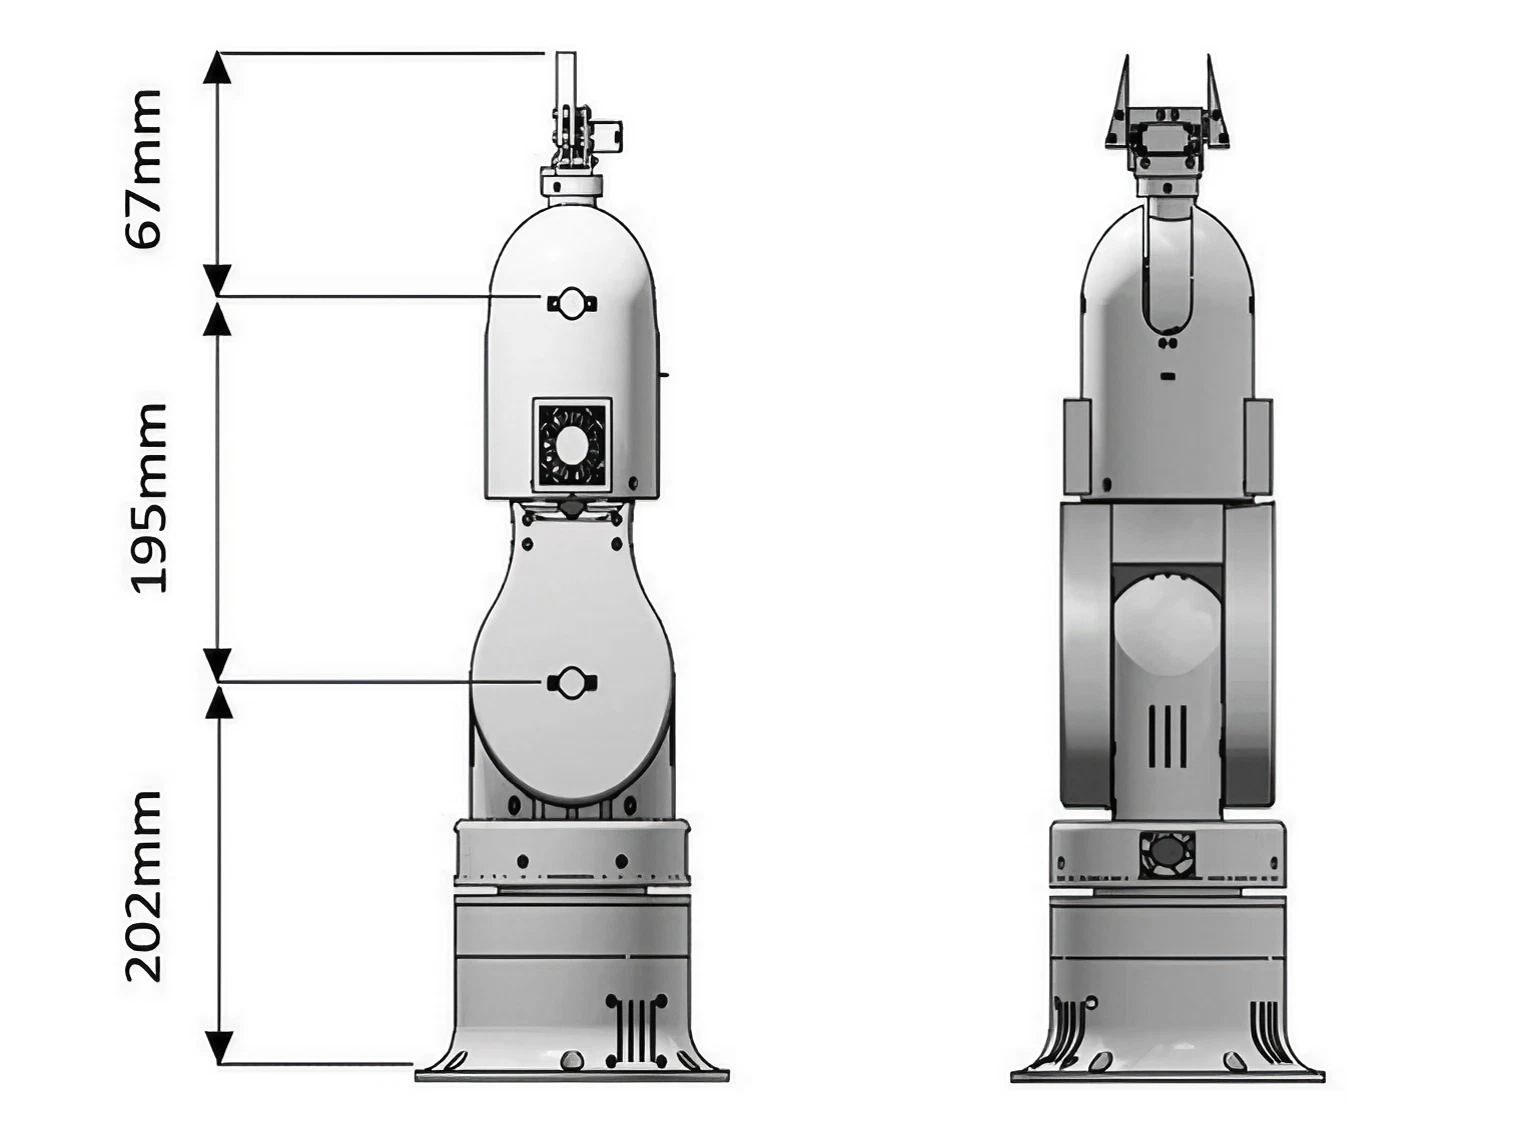
\includegraphics[width=8cm]{figs/uiarm.png}
        \end{center}
        \caption{Robot UIArm}
        \label{fig:uiarm}
    \end{figure}\ 
    
    A partir de la información proporcionada en este artículo, se han extraído los siguientes puntos fuertes:
    \begin{itemize}
        \item El diseño de las piezas se ha realizado mediante el uso de la herramienta de diseño \nameref{subsec:freecad}, esto supone una ventaja respecto 
        a \cite{KRIMPENIS2020103}, que utilizaba una herramienta privativa.
        \item Utiliza motores de pequeño tamaño con una reductora integrada, lo que aumenta su torque y abarata en gran medida los costes 
        del robot. Debido a esto, el consumo de energía es menor pudiendo hacer uso de una electrónica compacta y menos costosa.
        \item Al estar compuesto por menos piezas y tener pocos grados de libertad, se requiere menos tiempo para imprimir y construir este robot.
    \end{itemize}\
    Cabe destacar los siguientes puntos negativos:
    \begin{itemize}
        \item El espacio de trabajo (puntos del espacio alcanzables por el extremo del brazo) del robot es demasiado reducido. Esto es debido 
        a la disposición de los grados de libertad. Utiliza dos de ellos para cambiar la orientación del extremo del robot, dejando solo dos para el 
        posicionamiento, por lo que es imposible en la práctica abarcar todo el espacio 3D al alcance del brazo.
        \item Utiliza engranajes impresos en 3D para rotar la segunda articulación comenzando desde la base. Debido a esto, pierde exactitud en función 
        de la posición del brazo debido a la holgura de este tipo de transmisión.
        \item Carece de integración con \ac{ROS} y el autor no proporciona otro tipo de software que permita desarrollar programas para este robot perjudicando la 
        continuidad del proyecto.
    \end{itemize}\

    \item Existe un brazo robot impreso en 3D de 6 grados de libertad que ha ganado gran popularidad gracias a la plataforma 
    KickStarter \footnote{\url{https://www.kickstarter.com/projects/niryo/niryo-one-an-open-source-6-axis-robotic-arm-just-f/description}} en la cual fue 
    capaz de recaudar 80.000\euro \xspace de los 20.000 necesarios. 
    Este proyecto busca dar una alternativa de bajo coste al robot convencional usado por \textit{makers}, estudiantes y pequeñas compañías.\\
    Para lograr esto, apuesta por el uso de componentes comunes y la filosofía \textit{Open Source}. \\
    Aunque este modelo no es el más nuevo de la marca Niryo, si es el que más comunidad tiene y más extendido está.
    Este robot y los modelos posteriores, pueden ser adquiridos mediante la página oficial \footnote{\url{https://niryo.com/products-cobots/niryo-one/}}.
    \\
    \begin{figure} [ht!]
        \begin{center}
          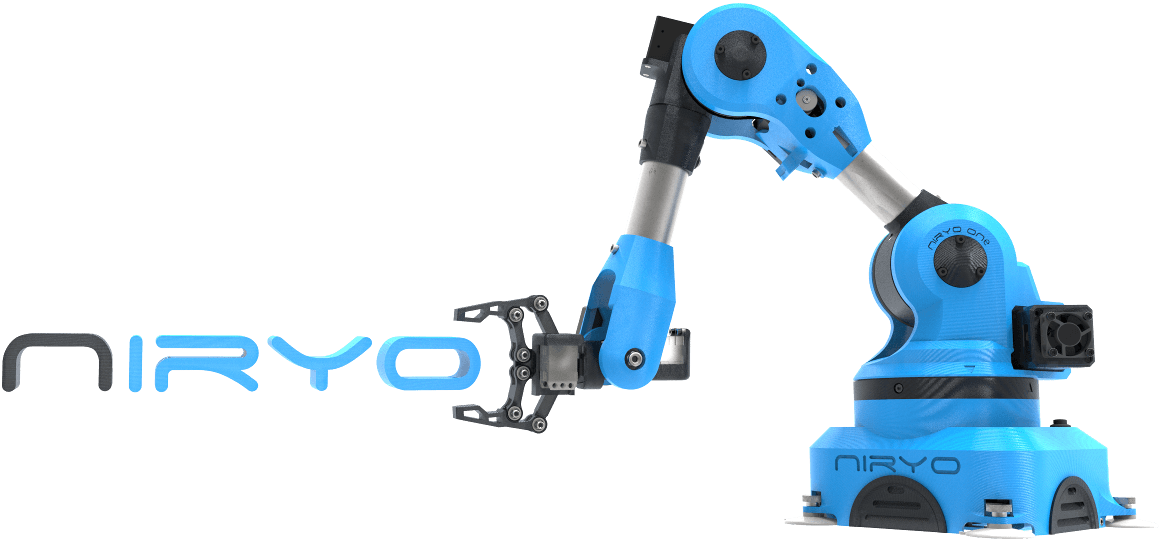
\includegraphics[width=11cm]{figs/niryo.png}
        \end{center}
        \caption{Robot Niryo One}
        \label{fig:niryo}
    \end{figure}\ 
    \newpage
    Este proyecto destaca positivamente por:
    \begin{itemize}
    \item El proyecto completo es de código abierto y se puede encontrar toda la electrónica necesaria y documentos para imprimirlo en 
    su repositorio de github \footnote{\url{https://github.com/NiryoRobotics/niryo_one}}.
    \item Tiene integración con ROS 1 y MoveIt.
    \item Cuenta con 6-DOF, lo que permite alcanzar gran cantidad de puntos con distintas orientaciones.
    \item Cuenta con una repetitividad de 0.5mm y puede levantar hasta 300g.
    \item Permite adaptar una gran variedad de herramientas diferentes.
    \item Es capaz de detectar colisiones gracias a sus motores codificados mediante sensores magnéticos.
    \end{itemize}
    En cambio, tiene los siguientes inconvenientes:
    \item Hace uso de una placa Raspberry Pi en vez de una placa Arduino/Esp32, lo que incrementa el coste del equipo. 
    \item Hablando del precio, el coste de este equipo comprado en su versión en aluminio ronda los 3500\euro. El coste de fabricación 
    de este robot mediante el uso de impresión 3D ronda los 1000\euro \xspace según este artículo \footnote{\url{https://www.zdnet.com/article/this-mini-industrial-robot-is-less-than-1k/}}
    \item Aunque proporcionan los ficheros fuentes del diseño, este ha sido realizado mediante SolidWorks\textsuperscript{\tiny\textregistered} por 
    lo que no puede ser editado sin tener que pagar por el programa.
    \item Pese a tener integración con ROS1, el proyecto no ha sido adaptado de forma oficial para ROS2, por lo que es necesario 
    usar un sistema operativo antiguo (Ubuntu 16.04) del año 2016. O bien utilizar Ros Bridge \footnote{\url{https://github.com/ros2/ros1\_bridge}} 
    para comunicar el ROS 1 de la placa con un  ordenador moderno con ROS 2.
   
    \newpage
    \item En el ámbito de los robots caseros, se puede destacar un referente reconocido, MeArm. Se trata de un 
    brazo mecánico de diseño simple y completamente \textit{OpenSource}, lo que significa que su código fuente y planos están disponibles 
    de forma gratuita para que cualquier persona interesada pueda acceder a ellos. De hecho, tal es su repercusión, que miles de personas 
    se han impreso el suyo o creado su propia versión mejorada. Prueba de ello es, la cantidad de modificaciones que se han ido subiendo a  
    páginas como Thingiverse\footnote{\url{https://www.thingiverse.com/search?q=mearm&page=1&type=things&sort=relevant}}. Además, existen 
    robots con diferentes nombres basados en el mismo concepto, como puede ser EEZYBotArm, una versión más robusta y atractiva que el original. \\
    Consta de 3 grados de libertad y de una pinza simple. Todos los motores del robots son servomotores de 9 gramos y se basa en el uso de 
    paralelogramos para transferir el movimiento de los motores al extremo del robot, manteniendo el peso de los mismos en la base. 

    \begin{figure} [h!]
        \centering    
        \subfigure[MeArm]{\label{fig:mearm}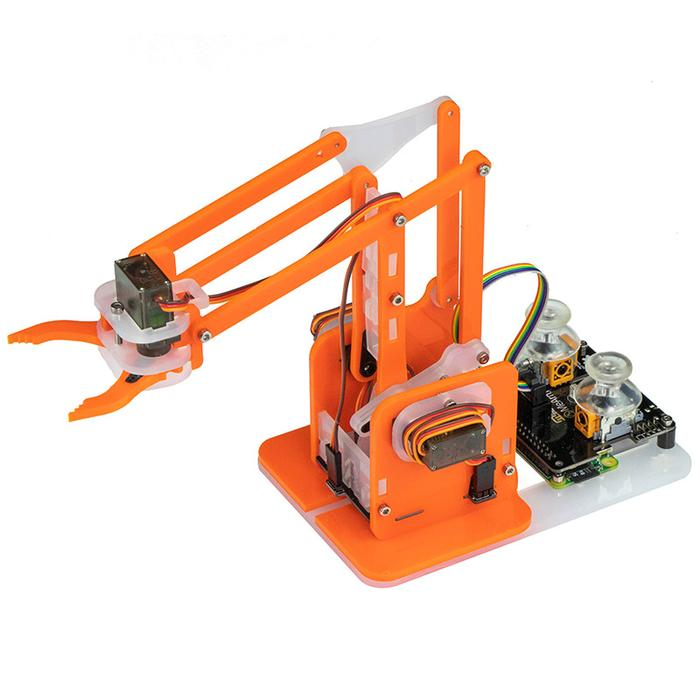
\includegraphics[width=0.3\linewidth ]{figs/mearm.jpg}}
        \hspace{3cm}
        \subfigure[EEZYBotArm MK1]{\label{fig:eezy}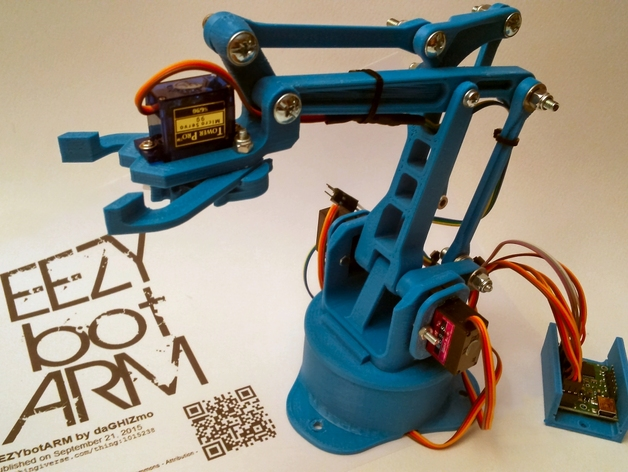
\includegraphics[width=0.3\linewidth]{figs/eezy.jpg}}
        \caption{Robots formados a partir de paralelogramos}
    \end{figure}
    
    Se trata de un proyecto muy extendido, con una comunidad que ha creado muchas variantes de él, por lo que para evaluar los puntos fuertes y 
    débiles del robot, se va a hacer referencia al robot original MeArm V1.
    Los aspectos significativos de este robot son:
    \begin{itemize}
        \item Se trata de un proyecto totalmente accesible y replicable, ya que usa pocos materiales y estos son fáciles de adquirir.
        \item El centro de masa del robot se concentra en la base, reduciendo la inercia del brazo y permitiendo así movimientos más rápidos.
        \item No requiere de apenas tiempo de impresión y el montaje es sencillo gracias a las numerosas guías de 
        montaje\footnote{\url{https://docs.rs-online.com/2bb1/0900766b81593e58.pdf}} que circulan por internet.
        \item Al usar servomotores, se puede establecer el ángulo de cada articulación fácilmente sin necesitar de ningún tipo de sensor externo.
        \item Debido a su forma y materiales utilizados, tiene un peso muy reducido pudiéndose acoplar a robots móviles sin afectar a 
        su rendimiento.
    \end{itemize}
    En cuanto a sus limitaciones, se deben mencionar:
    \begin{itemize}
    \item Se suele prescindir del uso de rodamientos en sus articulaciones. Esto reduce el tiempo de vida del brazo debido a que el propio rozamiento 
    de los ejes acaba desgastando el plástico, creando holguras que afectan directamente en la precisión. Esta holgura obliga a apretar en exceso los tornillos 
    que hacen de ejes de las articulaciones, aumentando el rozamiento y reduciendo fuerza útil de los pequeños motores.
    \item Este robot está limitado en cuanto a fuerza debido al uso de servomotores. Usa los típicos SG90 o similares con un torque de apenas 
    0.16 Newton-metro. El uso de servos más grandes aumenta significativamente el precio del dispositivo. 
    \item Los servomotores padecen de vibraciones al conectarle una carga. Esto hace que el conjunto tiemble en exceso durante los movimientos.
    \end{itemize}
\end{itemize}\
\vspace{1cm}
